\section{Introduction}
\label{sec:introduction}
A humanoid moving an object must coordinate its base, posture, arms, and hands while responding to the scene. The same instruction can require different trajectories depending on the object's location, the robot's stance, and its recent motion. Learning this behavior requires both perceptual grounding and a representation of how the whole body moves together. Vision--language--action (VLA) models transfer visual-semantic knowledge to control~\cite{rt2,openvla,pi0}, while world action models (WAMs) transfer visual dynamics from video generation~\cite{dreamzero}. Their application to humanoids~\cite{grootn1,psi0,motionwam,wholebodywam_wbc} motivates a complementary question: can the action generator itself inherit coordinated movement from motion pretraining?

We investigate \emph{Kinematic Action Models (KAMs)}: policies whose action-generating backbone is a pretrained motion generator. Motion pretraining captures articulation, root motion, and temporal coordination~\cite{mdm,kimodo}; policy adaptation grounds these structures in task instructions, visual observations, and measured robot state. This choice concerns the source of the generative prior, rather than prescribing a particular perception encoder. A KAM can receive visual or vision--language features while inheriting motion generation from a model trained in kinematic space. Figure~\ref{fig:routes} contrasts these backbone choices schematically.

\begin{figure}[t]
\centering
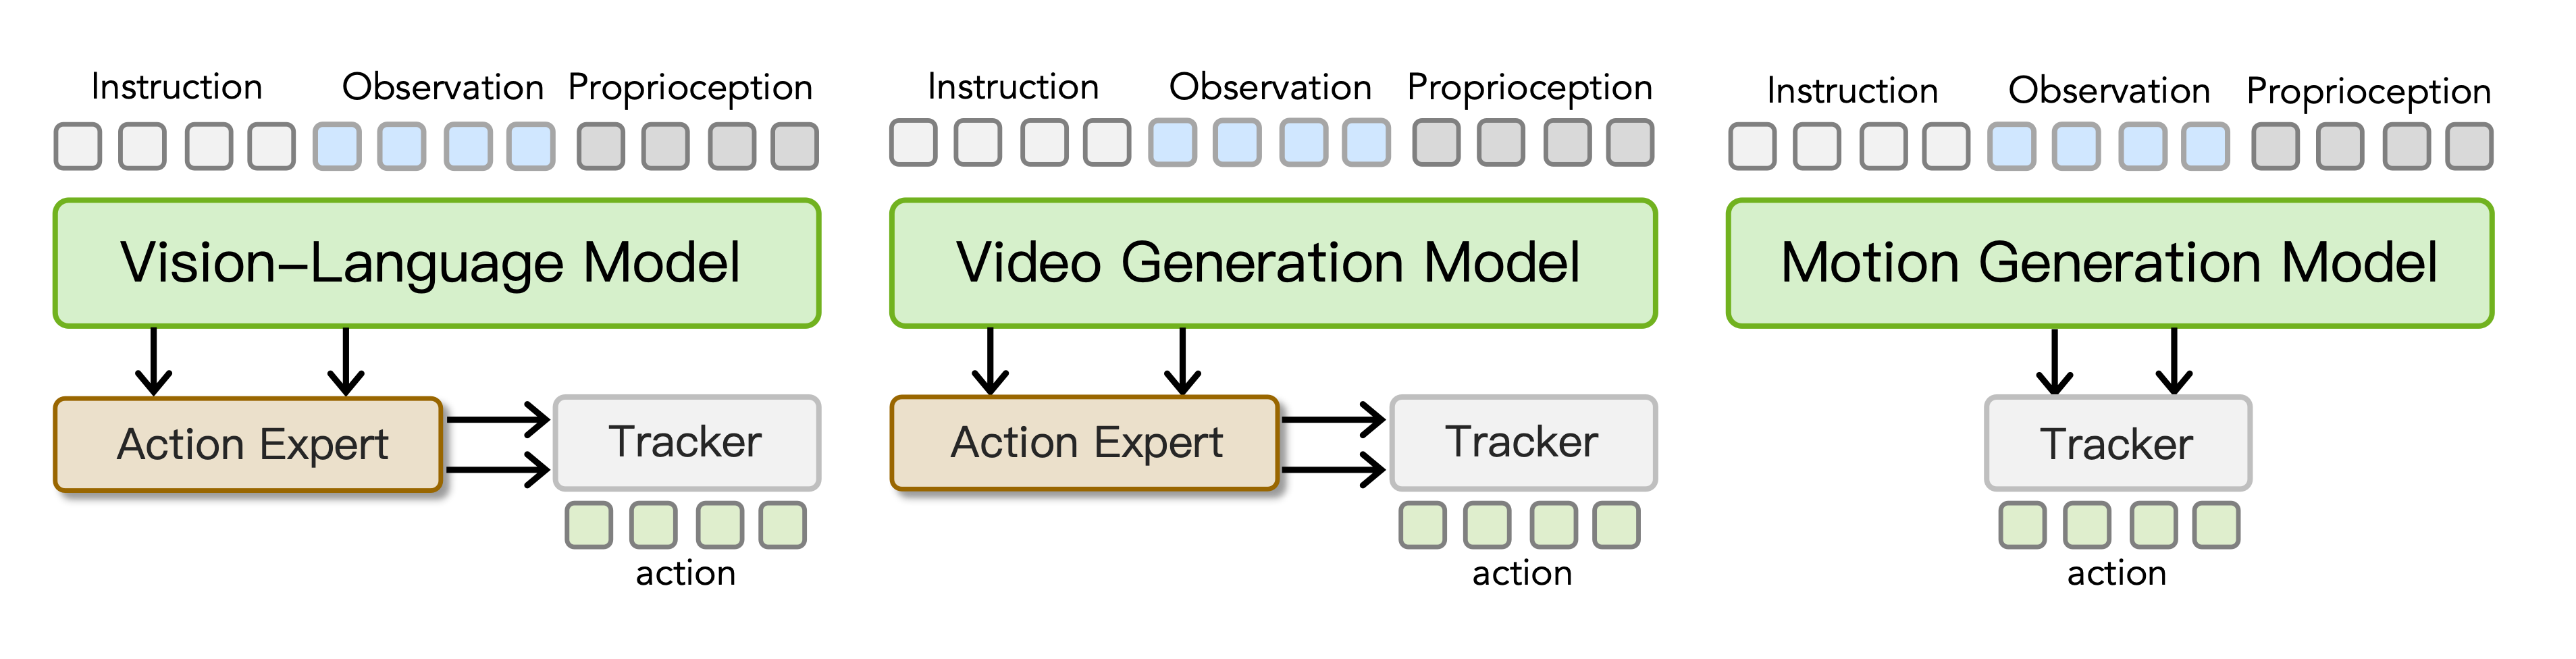
\includegraphics[width=\linewidth]{image/intro.png}
\caption{\textbf{Sources of pretrained structure for action generation.} Vision--language, video, and motion generators supply different priors. KAMs adapt a motion generator to predict kinematic references for a downstream tracker; perception grounds those references in the scene.}
\label{fig:routes}
\end{figure}

This approach separates two sources of supervision. Motion sequences, including human motion retargeted to a humanoid, can teach reusable movement structure without pairing every sequence with successful robot interaction and egocentric images. Robot demonstrations then teach how to condition this structure on the scene and task. The separation does not make a kinematic generator a controller by itself: its predictions must remain anchored to measured motion, respond to updated observations, and be executable through a tracking interface. The central adaptation problem is therefore to convert an offline sequence generator into a visually grounded, receding-horizon policy.

We instantiate this approach with \textbf{Kimodo-Policy}. It retains Kimodo's pretrained root and body denoisers~\cite{kimodo}, adds ControlNet-based visual branches~\cite{zhang2023adding}, and introduces a dedicated hand-control diffusion head. Root prediction conditions body articulation; future body features and visual context condition the hands. At every policy query, observed motion forms a constrained prefix, and the model completes a future chunk. Only a prefix of that chunk is executed before the next observation arrives. This connects the generator's temporal structure to closed-loop whole-body control through SONIC~\cite{sonic}.

Our evaluation distinguishes the pretrained \emph{motion backbone} from additional \emph{policy pretraining} on robot demonstrations. Both policy variants retain the same motion prior; only one initializes its conditioning modules and hand head with the 419-hour robot corpus. The pretrained policy achieves 72.14\% multi-task success on HumanoidArena and 60\% mean success on eight real-world tasks. On SIMPLE it is competitive with the strongest reported aggregate result, rather than uniformly superior on every task. Removing motion pretraining causes a large drop in a controlled ablation, whereas additional policy pretraining has task-dependent benefits, including a lower single-task HumanoidArena average. These distinctions delimit what the experiments establish.

Our contributions are threefold: (1) a concrete investigation of pretrained motion generation as the backbone of a visually grounded humanoid policy; (2) a root--body--hand adaptation mechanism combining visual residual conditioning, stage-specific gradient flow, and constrained history completion; and (3) evaluation across two simulation benchmarks and eight physical tasks, with controlled analyses of motion pretraining, policy pretraining, and model capacity.
